With every software engineering project comes the challenge of management with
respect to both time, development and personal resources. There are several
aspects to managing each and there are many ways to go about it. We have
obviously not had the luxury of a dedicated project manager who can take care of
planning tasks, handle communication, keep track of loose ends and continuously
assess the status of the project. Thus we have done this ourselves in parallel
with development which encourages a rigorous system that ``gets out of the
way'', while still providing a flexible work flow that supports the inevitable
change that is part of all software development; designs change as flaws are
discovered, inefficiencies must be optimized, refactoring of sloppy code is
required and so on.

We will first give a detailed presentation of the methods and tools we have used
and then evaluate how it went.

A management methodology that has become very popular among software developer
in recent years is the so-called agile method. It is based on the Agile
Manifesto\cite{agile-manifesto} which is a collection of twelve principles that
guides the method of work. The central focus is on response to change rather
than following a plan and working software rather than extensive documentation.

``Agile'' became so popular and widespread that it has now degraded to something
of a clich\'e that everyone seems to have their own definition of and is a
buzzword that is unavoidable in the industry. However, we find that it is still
a strong basis for project management and have chosen to use it for the
development of \thename{}.

\subsection{Phases and Iterations}
\label{sec:project-mgmt:phases}

The agile process works in a set of four phases from the inception of the
project to the transition into production. The following is a description of
each of the phases and what is to be the result of each. The phases are in
accordance with the work of Scott W. Ambler\cite{aup}.

\begin{description}
\item[Inception] is the initial phase of the project. The vision and scope of
  the product is identified and corresponding use cases are defined. An
  overarching development plan is laid out. The result of the inception is a
  so-called inception artifact which can be found in
  Appendix~\ref{appendecies:inception-artifact}.

\item[Elaboration] of the design and overall implementation is defined and the
  development plan is updated accordingly. The goal is to prove that the project
  can succeed and that the planned architecture will suffice.

\item[Construction] is the phase in which construction of the product takes
  off. Implementation of features happen in iterations (see below) and
  continuous evaluation of state and quality is applied.

\item[Transition] involves evaluating the result and deploying it to
  production. In our case the deployment is irrelevant since there is not
  anything or anyone to which we are delivering the product per s\'e.

\end{description}

The implementation is done in iterations of one to two weeks each, in which a
clear goal is defined for the iteration. At the end of each iteration the goal
is assessed and a new goal for the next iteration is defined. In this way
changes to both the fundamental ambition of the project and more concrete
details can be addressed in a very flexible way without ruining a master plan,
as would be the case if we were working under the \term{waterfall method}.

\subsection{Risk Assessment}
\label{sec:project-mgmt:risk-assessment}

The project involves a set of risks that characterizes potential pitfalls and
shortcomings that might be encountered during the course of design and
development. We have tried to capture them in the initial phase of the project
to be able to better cope with any such issues and hopefully avoid them
altogether.

The risk assessment has been established with inspiration from Dr. Wall\"uller's
paper ``Risk Management for IT and Software
Projects''\cite{risk-assessment}. Table~\ref{tbl:risk-assessment} is an excerpt
from the complete risk assessment which can be found in
Appendix~\ref{appendices:risk-assessment}.

\begin{table}[h]
  \centering
    \begin{tabular}{p{0.2\textwidth} p{0.7\textwidth}}
      \textit{Risk} & Fundamental design flaws \\
      \textit{Severity} & High \\
      \textit{Description} & The fundamental design could be found to not \textit{efficiently} solve the problems that it intents to. \\
      \textit{Preventive measures} & Continuous review and adjustment to the design must be applied. \\ \Xhline{2\arrayrulewidth}

      \textit{Risk} & Technical implementation difficulties \\
      \textit{Severity} & Medium \\
      \textit{Description} & It is a possibility that the complexity of the system will be a significant challenge in terms of actual implementation. \\
      \textit{Preventive} measures & Favor simplicity over optimization and follow to the \term{KISS} principle. Further accept that everything will most likely not be state-of-the-art and industrial strength software, but rather a proof-of-concept. \\ \Xhline{2\arrayrulewidth}

      \textit{Risk} & Platform dependencies \\
      \textit{Severity} & Low \\
      \textit{Description} & To facilitate efficient work flow we might have to depend on third-party libraries which do not work on some platforms, such as microprocessors and mobile devices. \\
      \textit{Preventive measures} & Evaluate whether a feature of the system can be implemented platform-independent or if it too much work compared to the benefits of using existing libraries that work on limited platforms.
    \end{tabular}
    \caption{Excerpt from risk assessment}
    \label{tbl:risk-assessment}
\end{table}

\subsection{The Backlog}
\label{sec:project-mgmt:backlog}

The tool that lays the foundation for the agile work flow is the backlog. It is
a collection of work that needs to be done ordered by priority. The work is
described in the form of stories which are small and optimally completely
independent chunks of work that can be processed separately.

Before any work is done on a story it is estimated in terms of the approximate
amount of work in involves. Points are awarded to each story resulting in an
overview of how much is done and how much is to be done at any given
time. Points can be given by any measure but for simplicity we have estimated
stories in terms of hours needed to complete the task.

Instead of having a single collection of all tasks we split the work into
categories such as ``Testing'', ``Documentation'', ``Design'' and ``Core
development'' and have essentially kept track of each category of work
separately. That enabled us to flexibly select which area of the project to
focus on.

\subsection{Tools}
\label{sec:project-mgmt:tools}

There are scores of tools available to aid in the agile management process. Some
are as simple as a to-do list manager, and some a full-blown management
suites. Given that we are only two people working on the project we decided to
``roll our own'' and use a Google Spreadsheet of which
Figure~\ref{fig:project-mgm:backlog} shows an excerpt.

\begin{figure}[h]
  \centering

  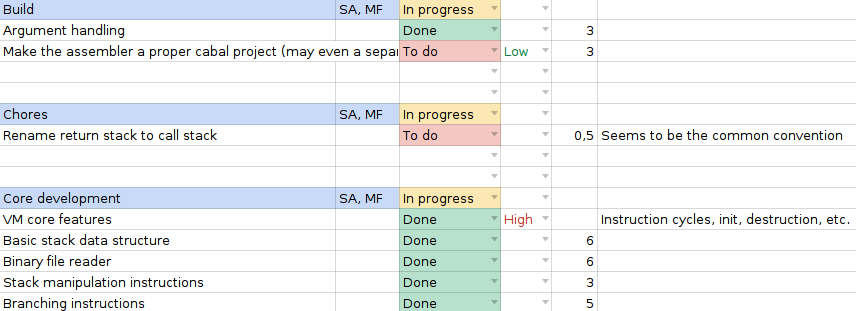
\includegraphics[width=.9\textwidth]{./images/backlog}

  \caption{Excerpt from the initial backlog}
  \label{fig:project-mgm:backlog}
\end{figure}

%TODO more?

\subsection{Technical Management}

When working in a team with multiple developers it is of paramount importance to
efficiently manage the codebase. When multiple people are writing code in the
same source tree it is virtually impossible to manually maintain and apply
changes from each other. Further it is an invaluable tool to be able to revert
changes and work on different branches of the system in a unified manner, which
is true for both a single person project and for dozens of developers of the
same codebase.

Specifically designed for this purpose are Source Code Management (SCM)
tools. Without going into excessive details, there two general forms of SCMs
which differ fundamentally in the way files can be edited concurrently. The
\textit{centralized} model (Microsoft TFS, Subversion) uses a central code
repository from which everyone edits files and is the single source of
truth. With \textit{decentralized} SCMs every developer has her own repository
and can merge changes from servers or other developers directly. There is no
single source of truth in this model, but a mainline tree is almost always
maintained.

The SCMs handle merging of files which have been edited by multiple people, and
are very good at doing this automatically. They can obviously not resolve merges
where the same lines of code have been changed differently, and so the developer
has to resolve the conflicting parts manually.

We have used the git\footnote{Git Source Control Management:
  \url{http://git-scm.com}} SCM tool together with the code hosting service
GitHub\footnote{\url{https://github.com}}. git is fully decentralized which we
find to be the most convenient model.

%TODO derp? more?

\subsection{Evalutation of the Management Process}

We followed the phase structure described in
Section~\ref{sec:project-mgmt:phases} starting with the inception phase and got
the vision and overarching plan of the project laid out. During the elaboration
we began to keep a backlog as concrete work started, both in terms design and
programming tasks. Programming tasks were fairly easy to describe and can be
well isolated, though many of them were inevitably interdependent and had to be
carried out in a specific order. However we quickly found that design tasks are
very difficult to describe in detail and even more so to estimate. This is both
due to the fact that describing a design task is essentially part of solving it,
and that the time it takes to figure out a design decision is highly
unpredictable. It becomes even more complicated when design flaws are discovered
and development plans must change. For several purposes it did not prove
beneficial to use the backlog strictly, but instead generated unnecessary
overhead, why we began to use it more ad-hoc.

As for planning of sprints we used the weekly meetings with our advisor as
milestones where we summarized the work that had been done and the plan for the
next week. That way we could get continuous feedback on the plan which was a
great help in taking the project in the right direction.

In the final weeks of the project we shifted from the spreadsheet backlog to
somewhat extensive to-do lists using a tool for the Emacs editor known as
org-mode\footnote{Org-mode for Emacs: \url{http://orgmode.org}} (for
organization mode). It enables nested lists of items with descriptions and
current status as well as tagging mechanisms. The main down-side of org-mode is
that it cannot be shared between the both of us, but because we were always
working at the same location it was not a significant issue.

We have certainly learned that good planning is vital for a successful project
process, and that it pays off to thoroughly weigh and examine design choices
before starting an implementation. It is a fine balance between management and
production and there will never be a single method that works for all types of
projects. We consider the essence of the agile methodology useful, but the
process must be tailored to each individual project. The concrete methods used
must depend of the type of software that is being developed, what the relation
to the end-user is, how it is going to be deployed (continuous delivery,
milestone based or a single one-time delivery), the size of the team and so
on. There is also a substantial difference between working for paying customers
and doing an academic project, the latter of which tends to change more than the
former as the project progresses.

%%% Local Variables:
%%% mode: latex
%%% TeX-master: "../report"
%%% End:
